\documentclass[review]{elsarticle}

\usepackage{lineno,hyperref}
\modulolinenumbers[5]
\usepackage{amsmath}
\usepackage[letterpaper, margin=1in]{geometry}
\usepackage{graphicx}
\usepackage{mhchem}
\usepackage{upgreek}
\usepackage{braket}

\newcommand\nt{\textup{\scriptsize{0}}}
\newcommand\total{\textup{\scriptsize{total}}}
\newcommand\el{\textup{\scriptsize{el}}}
\newcommand\inel{\textup{\scriptsize{inel}}}
\newcommand\elin{\textup{\scriptsize{el,in}}}
\newcommand\inelin{\textup{\scriptsize{inel,in}}}
\newcommand\out{\textup{\scriptsize{out}}}
\newcommand\PI{\textup{\scriptsize{PI}}}
\newcommand\noscat{\textup{\scriptsize{noscat}}}
\newcommand\sel{\textup{\scriptsize{1el}}}
\newcommand\elpl{\textup{\scriptsize{el,plural}}}
\newcommand\innoinel{\textup{\scriptsize{in,noinel}}}
\newcommand\signal{\textup{\scriptsize{signal}}}
\newcommand\inelpc{\textup{\scriptsize{inel,pc}}}
\newcommand\selpc{\textup{\scriptsize{1el,pc}}}
\newcommand\elplpc{\textup{\scriptsize{el,plural,pc}}}
\newcommand\Th{\textup{\scriptsize{Th}}}
\newcommand\KN{\textup{\scriptsize{KN}}}

\newcommand\elb{\textup{\scriptsize{el,\textit b}}}
\newcommand\inelb{\textup{\scriptsize{inel,\textit b}}}
\newcommand\elinb{\textup{\scriptsize{el,in,\textit b}}}
\newcommand\inelinb{\textup{\scriptsize{inel,in,\textit b}}}
\newcommand\outb{\textup{\scriptsize{out,\textit b}}}
\newcommand\PIb{\textup{\scriptsize{PI,\textit b}}}
\newcommand\noscatb{\textup{\scriptsize{noscat,\textit b}}}
\newcommand\selb{\textup{\scriptsize{1el,\textit b}}}
\newcommand\elplb{\textup{\scriptsize{el,plural,\textit b}}}
\newcommand\innoinelb{\textup{\scriptsize{in,noinel,\textit b}}}
\newcommand\inelpcb{\textup{\scriptsize{inel,pc,\textit b}}}
\newcommand\elplpcb{\textup{\scriptsize{el,plural,pc,\textit b}}}
\newcommand\innoinelpcb{\textup{\scriptsize{in,noinel,pc,\textit b}}}
\newcommand\selpcb{\textup{\scriptsize{1el,pc,\textit b}}}
\newcommand\inb{\textup{\scriptsize{in,\textit b}}}
\newcommand\inpcb{\textup{\scriptsize{in,pc,\textit b}}}

\newcommand\elf{\textup{\scriptsize{el,\textit f}}}
\newcommand\inelf{\textup{\scriptsize{inel,\textit f}}}
\newcommand\elinf{\textup{\scriptsize{el,in,\textit f}}}
\newcommand\inelinf{\textup{\scriptsize{inel,in,\textit f}}}
\newcommand\outf{\textup{\scriptsize{out,\textit f}}}
\newcommand\PIf{\textup{\scriptsize{PI,\textit f}}}
\newcommand\noscatf{\textup{\scriptsize{noscat,\textit f}}}
\newcommand\self{\textup{\scriptsize{1el,\textit f}}}
\newcommand\selff{\textup{\scriptsize{1el/f,\textit f}}}
\newcommand\elplf{\textup{\scriptsize{el,plural,\textit f}}}
\newcommand\innoinelf{\textup{\scriptsize{in,noinel,\textit f}}}
\newcommand\inelpcf{\textup{\scriptsize{inel,pc,\textit f}}}
\newcommand\elplpcf{\textup{\scriptsize{el,plural,pc,\textit f}}}
\newcommand\innoinelpcf{\textup{\scriptsize{in,noinel,pc,\textit f}}}
\newcommand\selpcf{\textup{\scriptsize{1el,pc,\textit f}}}
\newcommand\selfpcf{\textup{\scriptsize{1el/f,pc,\textit f}}}
\newcommand\inff{\textup{\scriptsize{in,\textit f}}}
\newcommand\inpcf{\textup{\scriptsize{in,pc,\textit f}}}

\newcommand\micron{$\upmu$m}
\newcommand\zpcf{\textup{\scriptsize{zpc,\textit f}}}
\newcommand\zpcb{\textup{\scriptsize{zpc,\textit b}}}
\newcommand\xzpc{\textup{\scriptsize{x,zpc}}}
\newcommand{\angstrom}{\mbox{\normalfont\AA}}

\journal{Ultramicroscopy}

%%%%%%%%%%%%%%%%%%%%%%%
%% Elsevier bibliography styles
%%%%%%%%%%%%%%%%%%%%%%%
%% To change the style, put a % in front of the second line of the current style and
%% remove the % from the second line of the style you would like to use.
%%%%%%%%%%%%%%%%%%%%%%%

%% Numbered
%\bibliographystyle{model1-num-names}

%% Numbered without titles
%\bibliographystyle{model1a-num-names}

%% Harvard
%\bibliographystyle{model2-names.bst}\biboptions{authoryear}

%% Vancouver numbered
%\usepackage{numcompress}\bibliographystyle{model3-num-names}

%% Vancouver name/year
%\usepackage{numcompress}\bibliographystyle{model4-names}\biboptions{authoryear}

%% APA style
%\bibliographystyle{model5-names}\biboptions{authoryear}

%% AMA style
%\usepackage{numcompress}\bibliographystyle{model6-num-names}

%% `Elsevier LaTeX' style
\bibliographystyle{elsarticle-num}
%%%%%%%%%%%%%%%%%%%%%%%

\begin{document}

\begin{frontmatter}

\title{X-ray microscopy for thick biological specimens}

%% Group authors per affiliation:
\author{Elsevier\fnref{myfootnote}\corref{mycorrespondingauthor}}
\address{Radarweg 29, Amsterdam}
\fntext[myfootnote]{Since 1880.}

%% or include affiliations in footnotes:
\author[mymainaddress,mysecondaryaddress]{Elsevier Inc}
\ead[url]{www.elsevier.com}

\author[mysecondaryaddress]{Global Customer Service\corref{mycorrespondingauthor}}
\cortext[mycorrespondingauthor]{Corresponding author}
\ead{support@elsevier.com}

\address[mymainaddress]{1600 John F Kennedy Boulevard, Philadelphia}
\address[mysecondaryaddress]{360 Park Avenue South, New York}


\begin{abstract}
We model the intensity fractions of beam components that are closely related to imaging quality for both X-ray and electron microscopy under the circumstance of a thick biological specimen. This not only allows one to gain clear perspective on the variation of image contrast with sample thickness, but also leads us to compare the radiation dose caused by X-ray and electrons with the usage of phase contrast and energy filter, where X-ray is found to cause less radiation damage than electron microscopy when the specimen thickness is beyond 1 - 3 \micron. 
\end{abstract}

\begin{keyword}
X-ray \sep electron \sep thick specimen \sep radiation damage
\end{keyword}

\end{frontmatter}

\linenumbers

\section{Introduction}

\section{X-ray interactions}

\paragraph{} The probability for a photon-matter interaction event (either scattering or photoionization) to occur over a fractional penetration depth \textit{dt} can be expressed as
\begin{equation}
P = \sigma_{i} \rho dt
\end{equation}
where $\sigma_{i}$ is the scattering cross section for interaction event \textit{i}, and $\rho$ is the sample density. This report is concerned with interaction events subdivided into elastic (Rayleigh) scattering, inelastic (Compton) scattering, and photoionization, with their cross sections respectively represented by $\sigma_{\el}$, $\sigma_{\inel}$, and $\sigma_{\PI}$. All cross section data are retrieved from \textit{Xraylib}, a multi-platform database for X-ray-matter interactions \cite{Schoonjans:2011km}. To tidy up the narrative, we also denote
\begin{align}
K_{\el} &= \sigma_{\el}\rho \\
K_{\inel} &= \sigma_{\inel}\rho \\
K_{\elin} &= \sigma_{\el}(1-\eta_\el)\rho \\
K_{\inelin} &= \sigma_{\inel}(1-\eta_\inel)\rho
\label{eq:inelin} \\
K_{\out} &= \sigma_{\el}\eta_\el\rho + \sigma_{\inel}\eta_\inel\rho \\
K_{\PI} &= \sigma_{\PI}\rho
\end{align}
where $\eta_\el$ and $\eta_\inel$ are the probabilities that a photon is scattered more than 90$^\circ$ (i.e., a photon that becomes undetectable, considering the case where an objective aperture is not present) in an elastic and inelastic scattering event, respectively. The two fractions can be found by integrating their corresponding differential scattering cross sections given by \cite{Sun:2015fr}
\begin{align}
\frac{d\sigma_\el}{d\Omega} &= \frac{d\sigma_\Th}{d\Omega}[F(x,Z)]^2 \\
\frac{d\sigma_\inel}{d\Omega} &= \frac{d\sigma_\KN}{d\Omega}[S(x,Z)]^2
\label{eq:kndiff}
\end{align}
where $d\Omega = 2\pi\sin\theta d\theta$ is the differential solid angle, and 
\begin{align}
\frac{d\sigma_\Th}{d\Omega} &= \frac{r_e^2}{2}(1+\cos^2\theta) \\
\frac{d\sigma_\KN}{d\Omega} &= \frac{r_e^2}{2}\Big[1 + k(1-\cos\theta)\Big]^{-2}\Big[1 + \cos^2\theta + \frac{k^2(1-\cos\theta)^2}{1+k(1-\cos\theta)}\Big]
\end{align}
are the differential Thomson and Klein-Nishina cross sections as a function of scattering angle $\theta$ and relative incident energy $k = E/m_e c^2$, assuming unpolarized radiation, given by Hubbell \cite{Hubbell:107568}. The atomic form factor $F(x,Z)$ and the incoherent scattering function $S(x,Z)$, both taking the momentum transfer $x = \sin(\theta/2)/\lambda(\angstrom)$ and atomic number $Z$ as parameters, also follow the definition by Hubbell, and are retrievable from \textit{Xraylib}. 

\paragraph{} A series of differential equations of x-ray intensity in various categories as a function of penetration depth $t$ can thereby be written \cite{Jacobsen:1998vj}:

\begin{itemize}

\item The intensity component due to photons that do not undergo any interaction with the sample, $I_{\noscat}$, is given according to
\begin{equation}
dI_{\noscat} = -I_{\noscat}(K_{\inel}+K_{\el}+K_{\PI}) dt.
\end{equation}
with initial condition $I_{\noscat}$(0) = $I_{\nt}$.

\item The component of photons that undergo only one elastic scattering event and remain in the detectable angular range, $I_{\sel}$, is given according to
\begin{equation}
dI_{\sel} = I_{\noscat}K_{\elin} dt - I_{\sel}(K_{\inel}+K_{\el}+K_{\PI}) dt
\end{equation}
with $I_{\sel}$(0) = 0.

\item For the component corresponding to photons undergoing multiple elastic scattering events yet still detectable, $I_{\elpl}$, the differential equation is
\begin{equation}
dI_{\elpl} = I_{\sel}K_{\elin} dt - I_{\elpl}(K_{\out}+K_{\inelin}+K_{\PI}) dt
\end{equation}
with $I_{\elpl}$(0) = 0.

\item For photons that are scattered out of the detectable angular range (backscattered), either elastically or inelastically, the corresponding intensity contribution $I_{\out}$ satisfies
\begin{equation}
dI_{\out} = (I_{\nt} - I_{\out} - I_{\PI})K_{\out} dt
\end{equation}
with $I_{\out}$(0) = 0.

\item For photons that are absorbed via photoionization, the component $I_{\PI}$ satisfies
\begin{equation}
dI_{\PI} = (I_{\nt} - I_{\out} - I_{\PI})K_{\PI} dt
\end{equation}
with $I_{\PI}$(0) = 0.

\item The portion of detectable photons that do not undergo inelastic scattering, i.e., the summation of $I_{\noscat}$, $I_{\sel}$, and $I_{\elpl}$, is denoted as $I_{\innoinel}$ and given by
\begin{equation}
dI_{\innoinel} = -I_{\innoinel}(K_{\inelin}+K_{\out}+K_{\PI})
\end{equation}

\item Lastly, $I_{\inel}$, the contribution of photons that undergo at least one inelastic scattering yet are still within the detectable angular range, is given in
\begin{equation}
dI_{\inel} = I_{\innoinel}K_{\inel} dt - I_{\inel}(K_{\out}+K_{\PI}) dt
\end{equation}
with $I_{\inel}$(0) = 0.

\end{itemize}

%\begin{figure}[!b]
%\begin{center}
%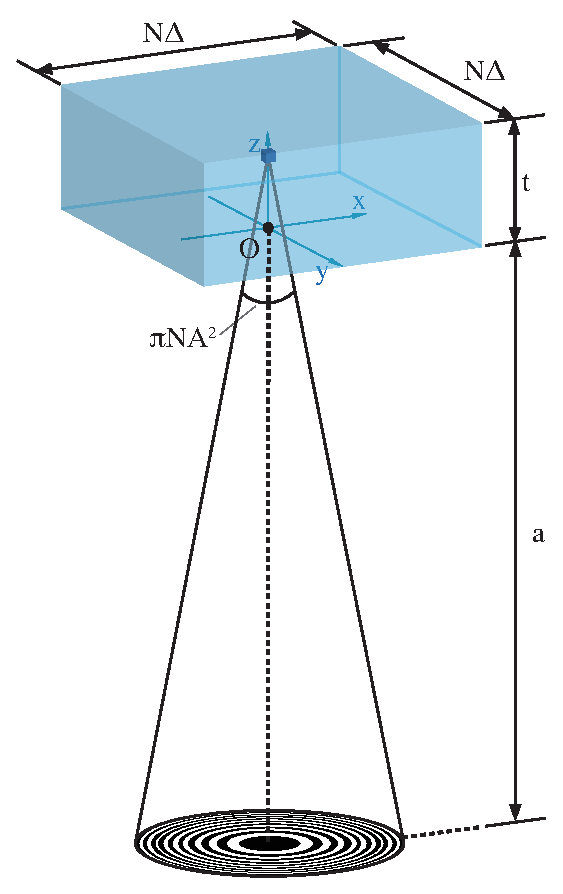
\includegraphics[scale=.6]{epsilon.eps}
%\caption{Illustration of the geometric model used for calculating $\epsilon$ for a sample with thickness $t$ and an imaging system with pixel size \textit{$\Delta$}, dimension of field of view $N$, and working distance $a$.}
%\label{fig:model}
%\end{center}
%\end{figure}

\paragraph{} Solutions to these differential equations yield
\begin{align}
I_{\noscat} &= I_{\nt}e^{-(K_{\inel}+K_{\el}+K_{\PI})t}
\label{x1} \\
\begin{split}
\label{x2}
I_{\sel} &= I_{\nt}K_{\elin}e^{-(K_{\inel}+K_{\el}+K_{\PI})t} \\
	&= K_{\elin}tI_{\noscat}
\end{split} \\
I_{\elpl} &= I_{\nt} \Big[ e^{-(K_{\out}+K_{\inelin}+K_{\PI})t} - (1+K_{\elin}t)e^{-(K_{\inel}+K_{\el}+K_{\PI})t} \Big]
\label{x3} \\
I_{\out} &= \frac{I_{\nt}K_{\out}}{K_{\out}+K_{\PI}} \Big[1 - e^{-(K_{\out}+K_{\PI})t}\Big]
\label{x4} \\
I_{\PI} &= \frac{I_{\nt}K_{\PI}}{K_{\out}+K_{\PI}} \Big[1 - e^{-(K_{\out}+K_{\PI})t}\Big]
\label{x5} \\
I_{\innoinel} &= I_{\nt}e^{-(K_{\inelin}+K_{\out}+K_{\PI})t}
\label{x6} \\
I_{\inel} &= I_{\nt}\Big[e^{-(K_{\out}+K_{\PI})t} - e^{-(K_{\inelin}+K_{\out}+K_{\PI})t)}\Big].
\label{x7}
\end{align}
It can be demonstrated that
\begin{equation}
I_{\noscat} + I_{\sel} + I_{\elpl} + I_{\out} + I_{\PI} + I_{\inel} = I_{\nt}.
\end{equation}

\paragraph{} In the specific case of X-ray phase contrast imaging, more useful categories can be lined out based on the above results. Firstly, the photons that constitute the image signals are, in addition to non-scattered photons, those having undergone single elastic scattering with the scattering angle within in the range defined by the numerical aperture (NA). Here we consider an NA required for 1 $\upmu$m resolution according to the Abbe criterion. The intensity of this portion of photons, $I_{\selpc}$, is related to $I_{\sel}$ by
\begin{equation}
I_{\selpc} = I_{\sel} \frac{\int_{0}^{s(2\theta=\it{NA})}I(s)ds}{\int_{\textup{forward}}I(s)ds}
\label{eq:frac1}
\end{equation}
where $s$ is the momentum transfer of scattering, $s$ = $4\pi\sin(\theta)/\lambda$, 2$\theta$ is the scattering angle, and $I(s)$ is the scattering intensity as a function of $s$. The upper integral is over the $s$ range stipulated by NA, while the lower is over the regime of forward scattering. We performed data fitting on the small angle X-ray scattering (SAXS) data of 80 different protein samples retrieved from Small Angle Scattering Biological Data Bank (SASBDB) \cite{Valentini28102014} to parameterize $I(s)$, where the normalized Guinier's law
\begin{equation}
I(s) = \exp(-\frac{1}{3}R_g^2s^2)
\label{eq:guinier}
\end{equation}
is applied to the portion with $s$ $<$ 1.3/$R_g$, while a polynomial approximation from the negative fourth to the zeroth order of $s$ is used to model the high-angle portion. $s$ = 3.0 is set as a cut-off point beyond which $I(s)$ is evaluated as 0 to take out the unphysical increasing part of the polynomial. This yields the integrable expression for $I(s)$ which can be plugged into Equation (\ref{eq:frac1}):

\begin{equation}
I(s) = 
\begin{cases} 
      \exp(-1.396s^2) & 0 \leq s < 0.311 \\
      0.0168s^{-4} - 0.1514s^{-3} + 0.4397s^{-2} - 0.2441s{-1} + 0.0399 & 0.311 \leq x < 3.0 \\
      0 & x \geq 3.0. \\
   \end{cases}
\label{eq:fit}
\end{equation}
Taking the $\pm90^{\circ}$-out-of-phase interfering amplitudes of $I_{\noscat}$ and $I_{\selpc}$ yields the signal intensity:
\begin{equation}
I_{\signal} = \sqrt{I_{\noscat}I_{\selpc}}.
\end{equation}

\begin{figure}[!t]
\begin{center}
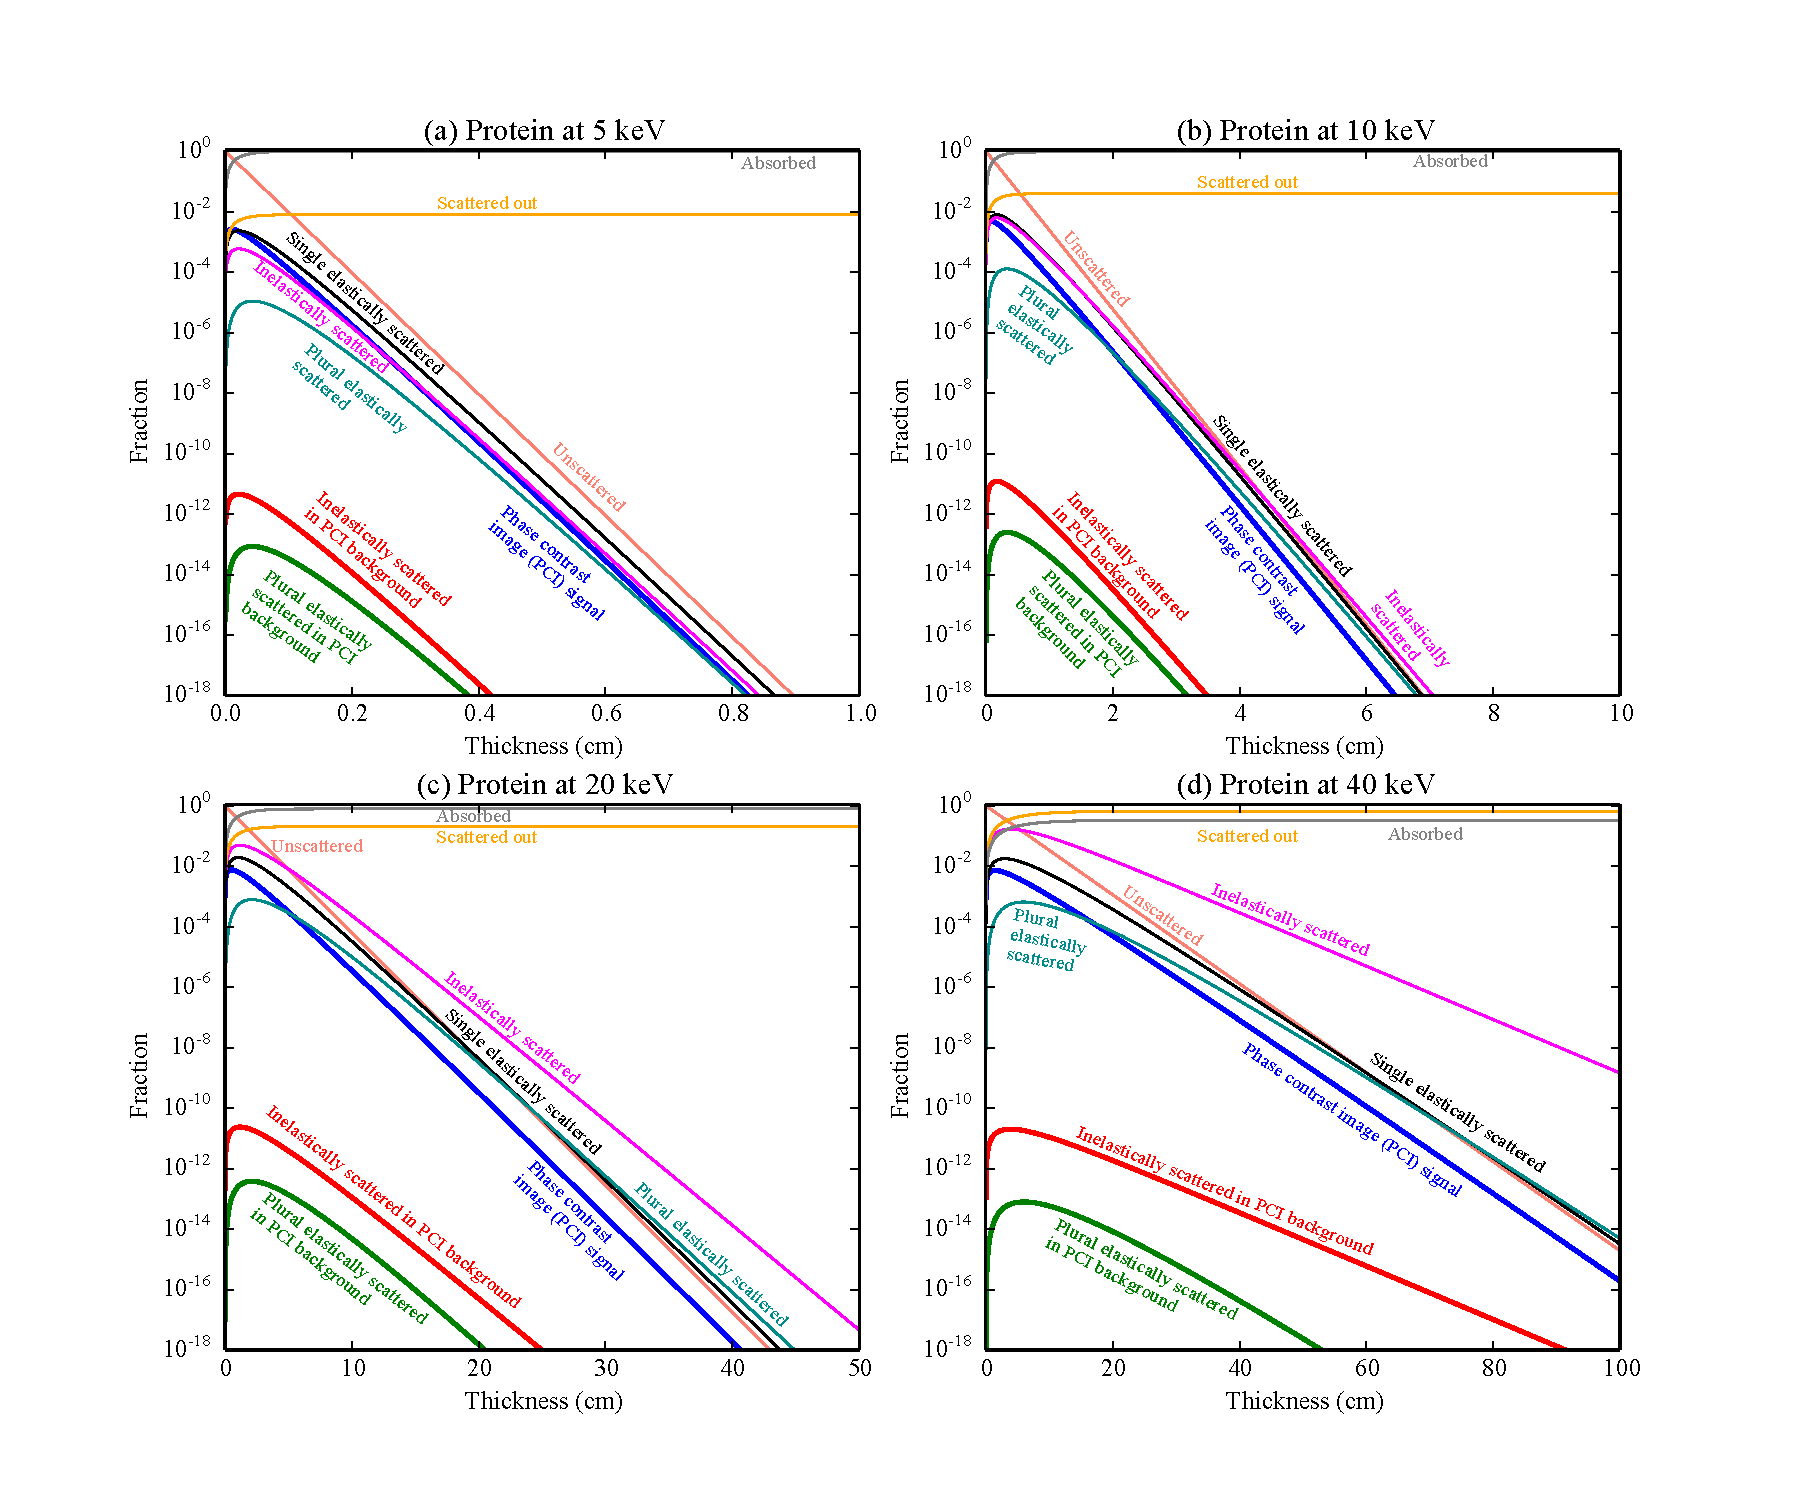
\includegraphics[scale=.6]{unimatrix_fig.pdf}
\caption{Normalized intensity profiles for X-ray in protein as a function of thickness at incident energy of (a) 5 keV, (b) 10 keV, (c) 20 keV, and (d) 40 keV.}
\label{fig:protein_x_cate}
\end{center}
\end{figure}

Furthermore, if one assumes that inelastic and plural elastic scattering events completely randomize the direction of photons, then the intensity of photons of such kinds that are collected by the objective and thus contribute to the background of phase contrast imaging, $I_{\inelpc}$ and $I_{\elplpc}$, can be calculated from $I_{\inel}$ and $I_{\elpl}$ purely on geometric basis:
\begin{align}
I_{\inelpc} &= I_{\inel}\frac{\pi (\it{NA})^2}{2\pi} \\
I_{\elplpc} &= I_{\elpl}\frac{\pi (\it{NA})^2}{2\pi}.
\end{align}
The above equations are based on the assumption that the working distance is much larger than the dimension of the field of view so the offset of the scattering center to the axis is negligible. 

\paragraph{} To simulate biological imaging, the sample is assumed to be a homogeneous block of protein with a composition of \ce{H_{48.6}C_{32.9}N_{8.9}O_{8.9}S_{0.6}} and a dry density of 1.35 \ce{g/cm^2}. This is the effective protein formula proposed by London through averaging over all 20 amino acids \cite{London:1989hh}. Figure \ref{fig:protein_x_cate} shows the intensity profiles relative to sample thickness at varying energies. 

\section{Electron interactions}

\begin{figure}[b!]
\begin{center}
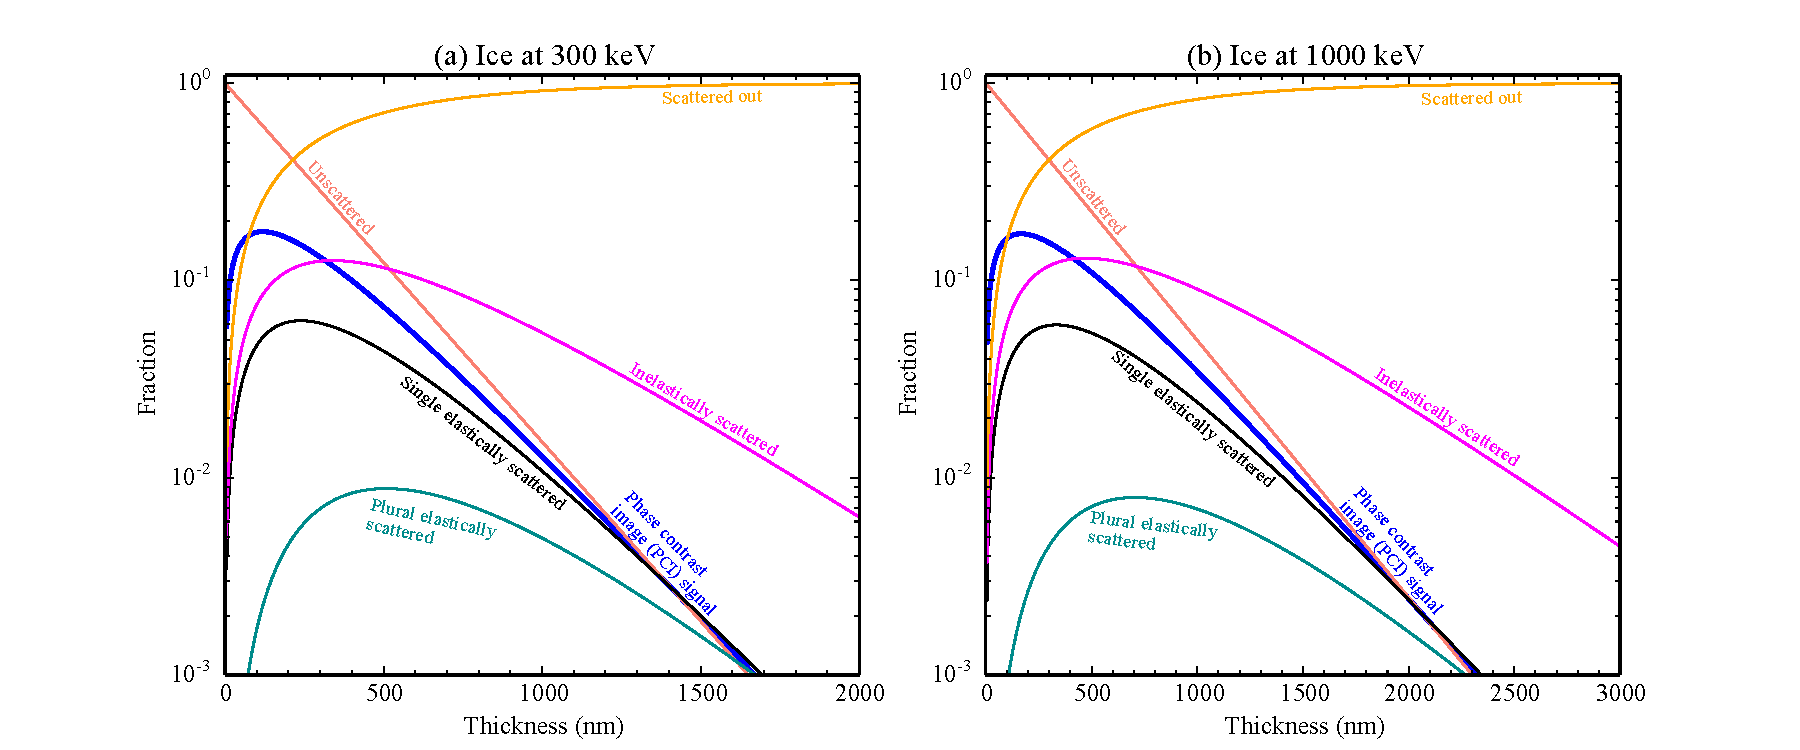
\includegraphics[scale=0.6]{unimatrix_fig_e.pdf}
\caption{Normalized intensity profiles for electrons in vitreous ice as a function of thickness at incident energy of 300 keV. Reproduced from Jacobsen et al. (1998) with permission.}
\label{fig:ice_e_cate}
\end{center}
\end{figure}

\paragraph{} It should be noted that electrons differ from X-ray in that they are never simply absorbed, which negates the presence of the absorption category. Moreover, now assuming that a typical objective aperture is present, one may make a general assumption on $\eta_\el$ based on a representative cutoff frequency of the aperture of $s_0$ = 4.12 $\mathrm{nm}^{-1}$ proposed by Langmore and Smith \cite{Langmore:1992kk}

\begin{equation}
\eta_\el \approx 1 - \frac{s_0}{10}.
\end{equation}
On the other hand, $\eta_\inel$ is simply assumed to be 0 as electron inelastic scattering is typically low-angle \cite{Williams:2006434}, so
\begin{align}
K_\out &= \sigma_\el \eta_\el \rho \\
K_\inelin &= \sigma_\inel \rho = K_\inel.
\end{align}
Equations \ref{x1} to \ref{x7} are then rewritten as
\begin{align}
I_{\noscat} &= I_{\nt}e^{-(K_{\inel}+K_{\el})}
\label{e1} \\
\begin{split}
\label{e2}
I_{\sel} &= I_{\nt}K_{\elin}e^{-(K_{\inel}+K_{\el})t} 
	\\ &= K_{\elin}tI_{\noscat} 
\end{split} \\
I_{\elpl} &= I_{\nt} \Big[ e^{-(K_{\out}+K_{\inel})t} - (1+K_{\elin}t)e^{-(K_{\inel}+K_{\el})t} \Big]
\label{e3} \\
I_{\out} &= I_{\nt} \Big(1 - e^{-K_{\out}t}\Big)
\label{e4} \\
I_{\innoinel} &= I_{\nt}e^{-(K_{\inel}+K_{\out})t}
\label{e6} \\
I_{\inel} &= I_{\nt}\Big[e^{-K_{\out}t} - e^{-(K_{\inel}+K_{\out})t)}\Big].
\label{e7}
\end{align}

\paragraph{} Based on the model, Jacobsen et al. \cite{Jacobsen:1998vj} have considered the case where a heavily hydrated specimen is embedded in vitreous ice. The ice layer is assumed to be so thick that one may use the scattering cross sections for \ce{H2O} throughout the entire sample. A reproduction of their work for electrons with energy 300 keV and 1000 keV is shown in Figure \ref{fig:ice_e_cate}. 

\section{Contrasting X-ray and electron microscopy on radiation dose}

\paragraph{} The categorization of X-ray and electron beam intensities would naturally shed light on the radiation dose done by probe beams to the specimen. In fact, the intensity breakdown is particularly useful for answering the dose question for electron imaging where absorption effect, which prevails in X-ray-matter interaction, is non-existent. As a paradigm scenario, we consider here a finer specimen model where protein features are dispersed as tablets in a layer of vitreous ice matrix with thickness $t_f$, on which another layer of ice with thickness $t_b$ ($t_b \gg t_f$) is overlaid, such that the specimen has a total thickness $t = t_b + t_f$ (Figure \ref{fig:contrast_scheme}). Jacobsen et al. \cite{Jacobsen:1998vj} have proposed a listing of equations describing the intensities of electrons passing through feature-containing columns ($I_f$) and matrix-only columns ($I_b$), respectively:
\begin{align}
I_{\noscatb} &= I_{\nt}e^{-(K_{\inelb}+K_{\elb})t}
\label{xb1} \\
\begin{split}
\label{xb2}
I_{\selb} &= I_{\nt}K_{\elinb}e^{-(K_{\inelb}+K_{\elb})t} \\ 
	&= K_{\elinb}t I_{\noscatb}
\end{split} \\
I_{\innoinelb} &= I_{\nt}e^{-(K_{\inelb}+K_{\outb})t}
\label{xb3} \\
I_{\elplb} &= I_{\innoinelb} - I_{\noscatb} - I_{\selb}
\label{xb4} \\
I_{\inb} &= I_{\nt}e^{-K_{\outb}t} 
\label{xb5} \\
I_{\inelb} &= I_{\inb} - I_{\innoinelb}
\label{xb7} \\
\end{align} % --------------------
and
\begin{align}
I_{\noscatf} &= I_{\nt}e^{-(K_{\inelb}+K_{\elb})t_b}e^{-(K_{\inelf}+K_{\elf})t_f}
\label{xf1} \\
I_{\self} &= (K_{\elinb}t_b + K_{\elinf}t_f) I_{\noscatf}
\label{xf2} \\
I_{\selff} &= K_{\elinf}t_f I_{\noscatf}
\label{xf2.5} \\
I_{\innoinelf} &= I_{\nt} e^{-(K_{\outb}+K_{\inelb})t_b} e^{-(K_{\outf}+K_{\inelf})t_f}
\label{xf3} \\
I_{\elplf} &= I_{\innoinelf} - I_{\noscatf} - I_{\self}
\label{xf4} \\
I_{\inff} &= I_{\nt}e^{-K_{\outb}t}e^{-K_{\outf}t}
\label{xb5} \\
I_{\inel} &= I_{\inff} - I_{\innoinelf}.
\label{xf7} \\
\end{align} % --------------------

\begin{figure}[htbp]
\begin{center}
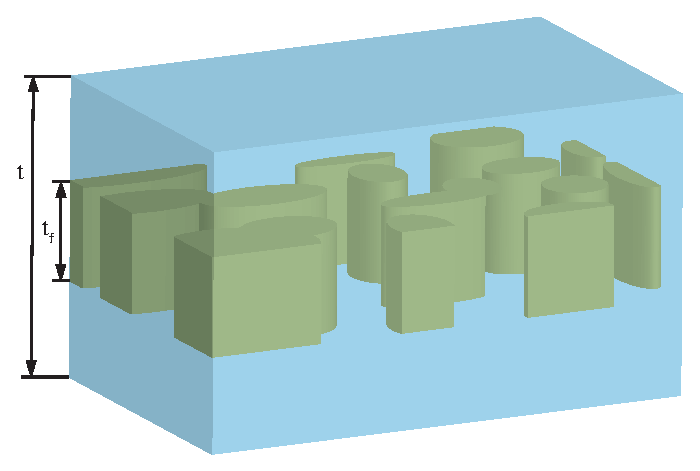
\includegraphics{contrast_scheme.eps}
\caption{Schematic diagram of the hydrated specimen model adopted for contrast computation. Protein features are assumed to be tablets dispersed within a layer of thickness $t_f$. Another layer of vitreous lies on the top with a much larger thickness $t_b$. In a parallel beam scenario, probe beams (X-ray or electron) traveling in columns containing proteins constitute image signals, while those passing through ice-only columns form the background. }
\label{fig:contrast_scheme}
\end{center}
\end{figure}

\paragraph{} From the matrix-feature dichotomy, the signal and noise of the resultant image can be straightforwardly written as 
\begin{align}
S &= N|I_f-I_b| \\
N &= \sqrt{N}\sqrt{I_f+I_b}
\end{align}
where $N$ is the number of probe particles per pixel. Consequently, the signal-to-noise ratio (SNR) is given by \cite{Sun:2015fr}
\begin{equation}
\begin{aligned}
\textit{SNR} &= \sqrt{N}\frac{I_f-I_b}{\sqrt{I_f+I_b}} \\ &= \sqrt{N}\Theta
\end{aligned}
\end{equation}
where $\Theta$ is the image contrast. For electron phase contrast imaging, this factor is expressed as
\begin{equation}
\Theta_{\mathrm{e,unfiltered}} = \frac{|I_{\innoinelf}-I_{\innoinelb}|+2\sqrt{I_{\noscatf}I_{\selff}}}{\sqrt{I_{\inff}+I_{\inb}}}.
\end{equation}
If an energy filter is used to screen out inelastically scattered electrons, the factor is modified as
\begin{equation}
\Theta_{\mathrm{e,filtered}} = \frac{|I_{\innoinelf}-I_{\innoinelb}|+2\sqrt{I_{\noscatf}I_{\selff}}}{\sqrt{I_{\innoinelf}+I_{\innoinelb}}}.
\end{equation}

\paragraph{} For X-ray, we only consider the case of Zernike phase contrast (ZPC), where phase-shifted X-ray beams interfere with a 90$^\circ$-shifted reference beam. In this case, it would be more convenient to exploit the wave nature of X-ray and utilize the linear absorption coefficients, $\mu_f = 4\pi\beta_f/\lambda$ and $\mu_b = 4\pi\beta_b/\lambda$, and phase advances, $\eta_f = 2\pi\delta_f/\lambda$ and $\eta_b = 2\pi\delta_b/\lambda$, where $\beta_{f/b}$ and $\delta_{f/b}$ are terms in the complex refractive index $n = 1 - \delta - \beta$ respectively for feature and matrix, to write \cite{Jacobsen:ZMiInRZY}
\begin{equation}
I_{\zpcf} \approx I_{\nt} e^{-\mu_b t_b}\Big[ 1 + 4\pi(\delta_f - \delta_b)\frac{t_f}{\lambda}\Big]
\label{eq:zpcf}
\end{equation}
and
\begin{equation}
I_{\zpcb} \approx I_{\nt} e^{-\mu_b t_b}.
\label{eq:zpcb}
\end{equation}
Equation \ref{eq:zpcf} and \ref{eq:zpcb} are based on the assumption that both materials are weak phase objects. Consequently, the contrast parameter for X-ray ZPC is given by
\begin{equation}
\Theta_{\xzpc} = 2\sqrt{2}\pi\frac{t_f}{\lambda}|\delta_f - \delta_b|\exp\Big(\frac{-\mu_b t_b}{2}\Big).
\end{equation}
It should be noticed that $\mu = K_{\total}$.

\paragraph{} According to the Rose criterion which states that a SNR of of at least 5 is required for precise identification of image features, $N$ should be
\begin{equation}
N = \frac{25}{\Theta^2}.
\end{equation}
It is further notice that, since for X-ray the probability of absorption almost always predominates over all interaction events, we can neglect the energy deposition due to inelastic scattering, and write the specimen radiation dose in Gray (J/kg) for X-ray as 
\begin{equation}
D_\mathrm{x} = \frac{NE}{\Delta^2 \Lambda_{\PIf} \rho}
\end{equation}
where $E$ is the incident photon energy, $\Delta$ is the pixel size (which defines the resolution in scanning X-ray microscopy), and $\Lambda_{\PIf} = 1/K_{\PIf}$ is the mean free path of X-ray with regard to absorption in the feature material. In the case of electron, the radiation dose is contributed by inelastic scattering only:
\begin{equation}
D_\mathrm{e} = \frac{N\Braket{E}}{\Delta^2 \Lambda_{\inel,f} \rho}
\end{equation}
where $\Lambda_{\inel,f}$ is analogous to its absorption counterpart, and $\Braket{E}$ is the expectation of energy deposition in an inelastic scattering event, evaluated from the electron energy-loss spectra (EELS) for ice as 46.0 eV and for protein as 37.5 eV \cite{Isaacson:1975wr}. In this work, we visualize the variation of radiation dose with the total thickness for a 10-nm-thick embedded protein layer, imaged with using soft (500 eV) and hard (10 keV) X-ray and 300 keV electrons with and without energy filter (Figure \ref{fig:dose}) for a spatial resolution of 10 nm. 

\begin{figure}[t!]
\begin{center}
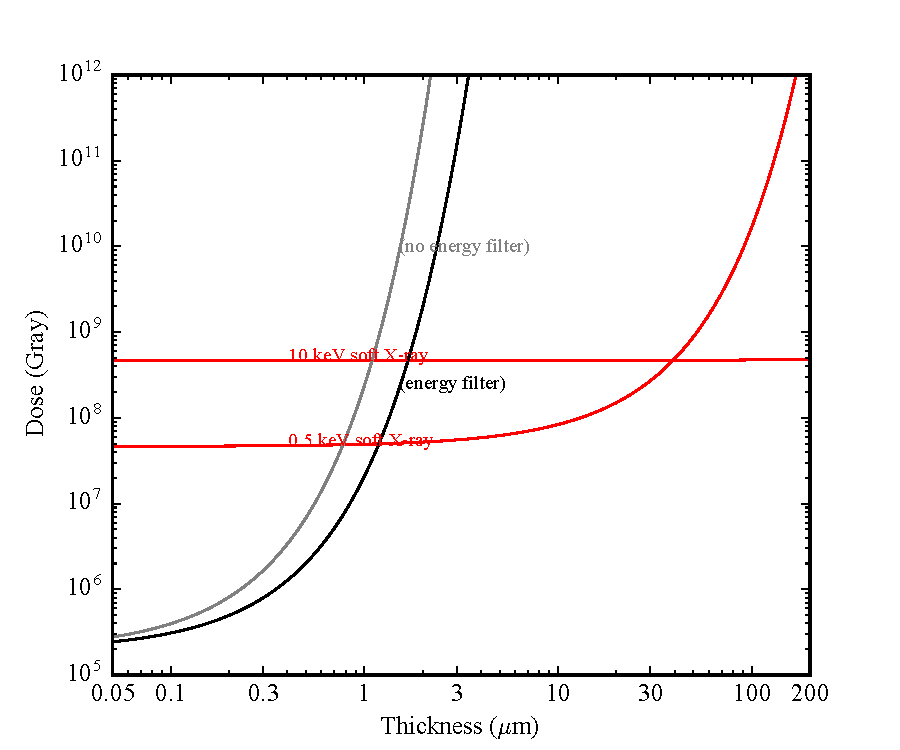
\includegraphics[scale=0.7]{dose.pdf}
\caption{Radiation dose at varying specimen thickness for 0.5 keV soft X-ray and 10 keV hard X-ray, in comparison with 300 keV electrons, with and without energy filter. Reproduced from Jacobsen et al. (unpublished) with permission.}
\label{fig:dose}
\end{center}
\end{figure}

\paragraph{} The paradigm scenario illustrated here indicates a general tendency that soft X-ray produces lower radiation dose than electrons. This advantage, however, is counterbalanced by the high spatial resolution that electron microscopy can provide, and diminishes when the specimen thickness is on or beyond the order of 10 \micron. Increasing the energy of X-ray would effectively reduce the sensitivity of radiation dose to ice thickness. Electron microscopy proves superiority for specimen thickness within the sub-100-nm regime; however, for thickness beyond 1 \micron, the ratio of multiple scattering or inelastic scattering over single elastic scattering events begins to take off, which, on the other hand, remains steady for X-ray. Thus, when spatial resolution is not a strict requirement, X-ray manifests to be a less intrusive technique for imaging biological specimens. 



\section{Acknowledgement}
\paragraph{} The authors would like to thank the developers and contributors of \textit{Xraylib} and SASBDB for supplying a substantial portion of the data used in this work. 

\section*{References}

\bibliography{mybib}{}

\end{document}